\begin{Hint}{2}
Considérer la symétrie axiale d'axe $(AC)$.
\end{Hint}
\begin{Hint}{3}
Attention, le calcul peut mener à des expressions qui \emph{semblent} différentes de celles demandées : il faut alors démontrer qu'elles coïncident avec les expressions demandées. Par exemple, on a $\sqrt{6+2\sqrt 5} = 1+\sqrt 5$. (Exercice : pourquoi ?)
\end{Hint}
\begin{Hint}{5}
On peut compléter la figure comme suit :
\begin{center}
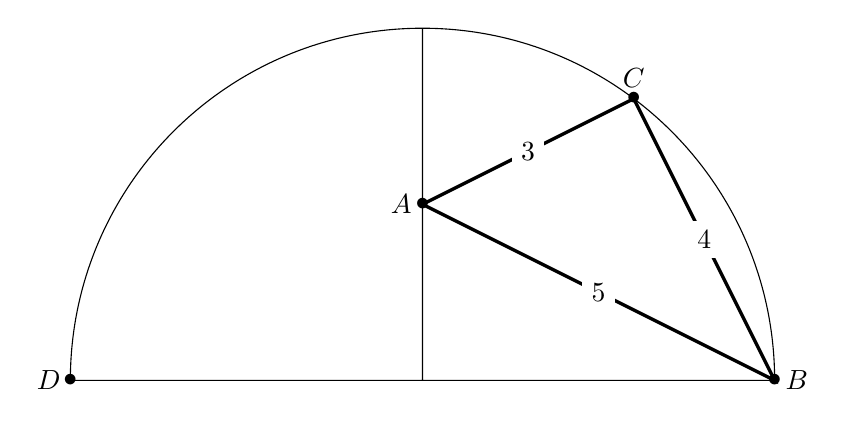
\begin{tikzpicture}[scale=1]
\draw (0,0) -- ({2*sqrt(5)},0) arc (0:180:{2*sqrt(5)}) node[left] {$D$} node {$\bullet$} -- (0,0) -- (0,{2*sqrt(5)});
\draw[very thick] (0,{sqrt(5)}) node {$\bullet$} node[left] {$A$}
-- ({2*sqrt(5)},0) node[midway,fill=white] {$5$} node {$\bullet$} node[right] {$B$}
-- ({3*2*sqrt(5)/5},{sqrt(5)+3/sqrt(5)}) node[midway,fill=white] {$4$} node {$\bullet$} node[above] {$C$}
-- cycle node[midway,fill=white] {$3$}  ;
%\draw ({-2*sqrt(5)},0)-- (0,{sqrt(5)});
\end{tikzpicture}
\end{center}
Ensuite, on peut prolonger la droite $(AC)$.
\end{Hint}
\begin{Hint}{8}
Il y a une hauteur $h$ que l'on peut calculer à l'aide de Pythagore.
Ensuite, si l'on note $H$ le pied de cette hauteur et $O$ le centre du cercle circonscrit, on peut par exemple appliquer Pythagore dans le triangle rectangle $OHB$.
\end{Hint}
\begin{Hint}{11}
Considérer les triangles $ADP$ et $AQB$
\end{Hint}
\begin{Hint}{13}
Appliquer Pythagore dans les triangles rectangles en partant du plus petit. Le résultat demandé est un nombre entier.
\end{Hint}
\begin{Hint}{14}
Pour calculer l'aire des deux lunules, il faut calculer l'aire du demi-disque de diamètre $[AB]$ et la retrancher à une autre aire.
\end{Hint}
\begin{Hint}{20}
Élever les trois quantités au carré.
\end{Hint}
\begin{Hint}{21}
Tracer le triangle (équilatéral) reliant les centres des trois petits cercles. Combien mesure  sa hauteur ?
\end{Hint}
\begin{Hint}{22}
La droite $(BC)$ recoupe le cercle en  un point $E$. Que dire de $[AE]$ ?
L'objectif est de calculer la distance $CE$, après quoi le rayon du cercle est relativement rapide à obtenir.

Autre indication : il y a une racine carrée dans la réponse.
\end{Hint}
\begin{Hint}{23}
La droite $(BC)$ recoupe le cercle en  un point $E$. Que dire de $[AE]$ ?
L'objectif est de calculer la distance $CE$, après quoi le rayon du cercle est relativement rapide à obtenir.
\end{Hint}
\begin{Hint}{24}
On peut trouver le centre en intersectant les médiatrices de deux cordes.
\end{Hint}
\begin{Hint}{25}
\end{Hint}
\begin{Hint}{26}
\end{Hint}
\begin{Hint}{27}

\end{Hint}
\begin{Hint}{28}

\end{Hint}
\begin{Hint}{29}
\end{Hint}
\begin{Hint}{30}
\end{Hint}
\begin{Hint}{31}
\end{Hint}
\begin{Hint}{32}
\end{Hint}
\begin{Hint}{33}
Élever les trois quantités au carré.
\end{Hint}
\begin{Hint}{34}
Tracer les centres des cercles et les relier.
\end{Hint}
\begin{Hint}{35}
Commencer par montrer que les deux premiers cercles, de diamètres $1/4$ et $1/9$, sont tangents. Dessiner leurs centres.
\end{Hint}
